\section{Scalability}

The blockchain trilemma, stated by Vitalik Butlerin tells us that, at the moment we can't have a blockchain that is scalable, decentralized and secure.
With those terms we mean:
\begin{itemize}
    \item decentralized: the blockchain system does not rely on a central point of control, so it is censorship resistant;
    \item scalable: the blockchain has the ability to handle an increasingly growing amount of transactions per seconds;
    \item secure: ability of the blockchain to operate as expected and defend from attacks.
\end{itemize}

Of course we have examples of blockchains with two out of three:
\begin{itemize}
    \item decentralized and secure: bitcoin and ethereum for example, they are not scalable however;

    \item secure an scalable: hyperledger which is not decentralized at all, but is secure because under a single administrative domain;

    \item scalable and decentralized: EOS, NEO with a minimal censorship resistance because a few nodes control the network.
\end{itemize}
Algorand is actually trying to solve the trilemma.

There are many solutions to scale blockchains, but all of them neglect the decentralization, for example:
\begin{itemize}
    \item delegated proof of stake: the network selects 21 nodes that will choose the next block for all the network, those nodes will be trusted by definition so it's more like a semi-decentralized solution;

    \item proof of work: it tend to create large mining pools which basically centralize the mining power, a lot far than initial Nakamoto intentions.
\end{itemize}

\subsection{Scalability problems}
Bitcoin transfer is too slow because the network adds 1 block every 10 minutes and in order to have a full confirmation you have to wait for 6 blocks, so a payment takes on average an hour to be verified.
Bitcoin has high transaction fee even though we are waiting so long for the verification.
Bitcoin does not scale because a block has a fixed size and so it can't take many transactions in it, for example for a block size of 1MB and a transaction of 250 bytes we have 400 transactions every 10 minutes, which means at maximum 7 transactions per second, in comparison VISA supports 45000 tps peaks.

\subsection{On chain solutions}
We could think to increase the block size, however larger blocks takes longer to propagate, it's like centralization.
We could increase block rate but this will raise the number of forks making the system less secure.
We could think of switching the consensus protocols but, altough the low energy cost, highly scalable and fast transactions and the complete deletion of 51\% attack we are kinda centralizing the network, so it's not so convenient.

\subsection{Off-chain solutions}
The last thing we can do is to build cross-chains or side-chains: we break the blockchain into a set of segments and implement some communication among chains.

\subsection{Channels}
One of the various ideas for off-chain payment is the \emph{off-chain payment channels}: allows us to not broadcast all transactions on the network doing most transactions off-chain, and use the blockchain as arbiter only if necessary.

The idea is to create a separate channel in which make various transactions, then at the channel closing we write on the blockchain the outcome of all of those transactions.
Basically blockchain is used for settlement while the transactions happen directly at the network speed.
This idea can be implemented on existing infrastructure in a decentralized, trustless way, allowing high volumes and instant micro-payments.

Bitcoin Lightning Network was released in alpha version in January 2017, in January 2018 the first known purchase through this network was done, while Ethereum Raiden Network (uRaiden) was launched on Ethereum mainnet in November 2017.
Both of them are example of payment channels, we will see the lightning network.

Channels in a blockchain form a layer 2 above the blockchain but are extremely scalable.

\section{Basic tools for layer-2 channels}
\subsection{Multisignatures in Bitcoin}
In Bitcoin transactions can use multisignature addresses which are bitcoin associated to a multisignature address.
Basically there are bitcoins locked to multiple public keys, that usually belongs to different people, so it's a ledger owned by more than one person.
Based on the type of application in order to unlock those coins you need the signature from some or all of the public keys, so some or all of the associated people.

It's implemented through the \verb|CHECKMULTISIG| script of Bitcoin (also known as Pay-to-multisignature \verb|P2MS|) which requires to include a set of different public keys and a subset of the corresponding private keys to be redeemed.
The said script is generically implemented in the form \verb|m-of-n multisig| which means that out of $n$ public keys it requires $m$ valid signatures.
It's implemented using the locking script in the form: \verb|m <pubkey 1> ... <pubkey n> n CHECKMULTISIG| while a valid unlocking script is in the form \verb|<sign 1> ... <sign m>|.

Some practical examples are:
\begin{itemize}
    \item 1-of-n: anyone of $n$ different parties can approve the transaction, like the management of a company;
    \item 2-of-2: each of the separate parties must approve the transaction;
    \item 2-of-3: any two out of three parties can approve the transaction.
    It's most famous application is the \emph{escrow contract} in which two counterparts engage a third party to act as an arbitrator ni the event of a dispute.
\end{itemize}

\subsubsection{Escrow transactions}
Alice wants to buy something from Bob and they live in different cities, so there is no possibility of direct goods exchange.
Bob promises to ship the book upon receiving Bitcoin payment but Alice does not trust Bob, so both of them do not trust each other.

In order to solve the problem both of them can introduce a third party and make an escrow transaction.
They engage Judy to solve a possible dispute but without giving her the funds, so basically during the course of the transaction no one can actually move the funds on it's own without the participation of at least one of the other two.

The algorithm is:
\begin{itemize}
    \item Alice creates a 2-of-3 multi signature transaction using her address as input address while the output contains one public key from each Alice, Bob and Judy.
    \item Alice publishes the transaction on the blockchain;
    \item coins are \emph{held in escrow} and any two of them can redeem the bitcoin and specify the receiver of the bitcoins;

    \item if the actual shipping goes smoothly Alice and Bob can jointly sign and release the funds to Bob without Judy's involvement.
    It only needs one extra transaction on the blockchain;
    \item If otherwise there is a dispute of any kind both Alice and Bob can contact Judy which will decides which of the two cheated and then she can:
    \begin{itemize}
        \item signs a transaction with Alice sending the money from escrow back to Alice;
        \item signs a transaction with Bob in order to terminate the transaction.
    \end{itemize}
\end{itemize}

\subsubsection{Problems with multi-signatures}
In order to make a multi-sig transaction you need to have the pubkey of the receivers, this implies:
\begin{itemize}
    \item the receivers needs to release those informations to the public;
    \item the customer need special bitcoin wallet software to create a custom multisig transaction script;
    \item the resulting transaction is five times larger than a normal transaction (5 pubkey instead of 1) so fees should be higher in order to be considered from the miners.
\end{itemize}

\subsubsection{Pay to script hash}
A solution for multi-sig scripts (and generally complex bitcoin scripts) is to include the hash of the script, instead of the script, in the locking script.
In order to unlock and redeem the transaction, the receiver presents the original script that produces the same hash contained in the locking script and the signatures:
\begin{itemize}
    \item the locking script becomes: \verb|OP_HASH160 <RedeemScriptHash> OP_EQUAL|;
    \item the unlocking script becomes: \verb|<ResponseToRedeemScript> <RedeemScript>|
\end{itemize}

\subsection{Hash/hash-time locked contracts}
There exists special kind of scripts with a complex redeeming condition:

\subsubsection{Hash lock}
Hash a secret and store it publicly in a script (or a smart contract).
In order to unlock it the intended recipient of the funds must provides the secret publicly.

\subsubsection{Hash Time lock}
Hash a secret and store it publicly in a script (or a smart contract), in order to unlock it:
\begin{itemize}
    \item the recipient must provide the secret publicly;
    \item wait for a timeout specified in the script.
\end{itemize}

\subsection{Atomic swaps}
Hash time locked contracts (HTLC) are used in payment channels like the Bitcoin Lightning Network but also to implement atomic swaps.
Let's suppose we want to exchange one cryptocurrency for another, we can go to an exchange, make our offer and find someone interested.
In order for the exchange to happen the user must send it's funds to the receiver's address but this way the receiver must be trusted.

Atomic swap is a technology that allows to perform p2p exchanges without the need of a third party, using HTLC.
Let's assume Alice has some Bitcoins and Bob some ZEN and they agreed on exchanging some amount one another:
\begin{itemize}
    \item Alice then creates a HTLC on the bitcoin blockchain forging a secret and disclosing it's hash only into the locking script;
    \item Bob on the other side creates a similar contract on the ZEN blockchain with the same hash disclosed by Alice;
    \item when Alice will redeem the ZEN token she must publicly disclose the secret in order for the unlocking script to actually works;
    \item since the secret now is public on the ZEN blockchain, Bob can look it up and go to redeem its bitcoins.
\end{itemize}
From both side if nothing happens for 24 hours the money will return back to it's first owner because of the timelock component of the HTLC, also the contract cannot be force because the secret is secret and hash is a one-way function.

An example of HTLC script in Bitcoin is:
\begin{verbatim}
    OP_IF
        OP_SIZE
        AddInt64(secretSize)
        OP_EQUALVERIFY
        OP_SHA256
        AddData(secretHash)
        OP_EQUALVERIFY
        OP_DUP
        OP_HASH160
        AddData(pkhThem[:])
    OP_ELSE
        AddInt64(locktime)
        OP_CHECKLOCKTIMEVERIFY
        OP_DROP
        OP_DUP
        OP_HASH160
        AddData(pkhMe[:])
    OP_ENDIF
    OP_EQUALVERIFY
    OP_CHECKSIG
\end{verbatim}
in which we can see the first branch of the if dedicated to the hash lock to Bob while the else branch dedicated to the time lock to Alice.

\subsection{Data Registering}
The irreversibility of the blockchain can be exploited beyond payments, for example we could compute a digital fingerprint of a file and record it on the blockchain and enstablish a \emph{proof of existence} of that file on a specific date (bound to the block number and it's timestamp).
We can use the blockchain as a notary ledger.

In order to do this we can use the output destination address as a free-form 20 byte generic field generating a fake payment which cannot be spent because no private key corresponds to that address, so cannot be redeemed.

This means that the corresponding entry in the UTXO can never be removed which cause data pollution because the RAM size of the UTXO increases.

To solve this problem after 2013 a new instruction is introduced: \verb|OP_RETURN <data>| which instructs the blockchain to invalidates the script whatever code in the unlocking script, this way corresponding bitcoins can never be spent.
So we can add arbitrary data after that instruction in order to add arbitrary data to a Bitcoin transaction.
It is mainly used in two cases:
\begin{itemize}
    \item transactions with dummy outputs in which no bitcoins are spent, but only to register data on the blockchain;
    \item burn bitcoin: it's called proof-of-burn script and bitcoins in this script can never be redeemed, and it's provable that those bitcoins have been destroyed.
    It's mainly used to bootstrap an alternative cryptocurrency by forcing people to destroy bitcoin to gain fresh coins in the new cryptocurrency, but also to implement an alternative form of consensus: burn coin to win the lottery, the more coins you burn, the highest is the probability you have to win, instead of paying energy with PoW you pay with coins.
\end{itemize}

\section{Bitcoin lightning network}
Let's start from an analogy: a customer gives the credit card to the bartender and starts ordering drinks, the bartender notes the drinks on a tab but does not charge credit card immediately.
This way we can avoid to pay credit card fees every time the credit card is run taking the balance until the end and settling up at one point.
There is no risk for the bartender because he holds the customer credit card and if the customer disappear he still has a warranty.

\subsection{General idea}
We can think of the Lightning Network as similar situation: instead of giving the credit card to the bartender the customer deposit some credit into an address called payment channel, then the payments are not registered on the blockchain as transactions but only on private ledgers managed by the bartender.
So every time a customer drinks a new beer the bartender sends a new transaction which replaces the previous one, this way both endpoint can keep track of the transaction but not change the ledger and many transactions can be sent without paying any fee.

We can notice that the bartender risks nothing because he can commit the transaction on the blockchain at anytime and redeem it's money.
So in general we have private ledgers which take into accounts some transactions which are not yet sent to the blockchain and at some point the settlement will happen.
Moreover this approach also increases privacy because the blockchain has a record only of the opening and of the closing transaction.

As we described the protocol up to now for a user Alice who wants to buy stuff from various market she has to create $n$ different channels, one for each party, but opening and closing channels requires an expensive transaction on the layer-1 Bitcoin network.
We can leverage third parties: if Alice already has a channel with Charlie and Charlie has an open channel with $Bob$, then Alice can create a Bitcoin script saying that she will pay Charlie only if Charlie paid Bob.

\subsection{Technically}
It's a layer-2 protocol proposed by Poon and Dryja, channels can be unidirectional or bidirectional and a channel is a structure defining the following operations:
\begin{itemize}
    \item \verb|channel opening|;
    \item \verb|offchain commitments|;
    \item \verb|channel closing|;
\end{itemize}
and only the opening and closing transactions are registered on the blockchain.
Also if one of the user involved in the channel tries to cheat there is a punishment: all the channel funds are granted to counterparty, because if an old commitment is published by one cheating party, it will be invalidated by the other party publishing a remedy script.

Basically a payment channel is a 2-user multi-signature address, this way it requires the signature of both Alice and Bob to spend the money in it.
The \emph{channel opening} is a funding transaction in which Alice sends money to the multisignature address taking the money from one of her addresses, this transaction of course has to be registered to the blokchain in order to start.

Alice and Bob then start to transact through commitment unconfirmed transactions:
\begin{itemize}
    \item the source address is the multi-sig funded address
    \item the destination address is both Alice and Bob's addresses, splitted based on the settle up of all the transactions;
    \item those transactions are exchanged only between Alice and Bob, not broadcasted to the network, this way each party has a local picture of the balances.;
    \item each of those transactions is signed both by Alice and Bob, and stored locally
\end{itemize}
For example: Alice sends 80 BTC to Bob, so a transaction is issued:
\begin{figure}[H]
    \centering
    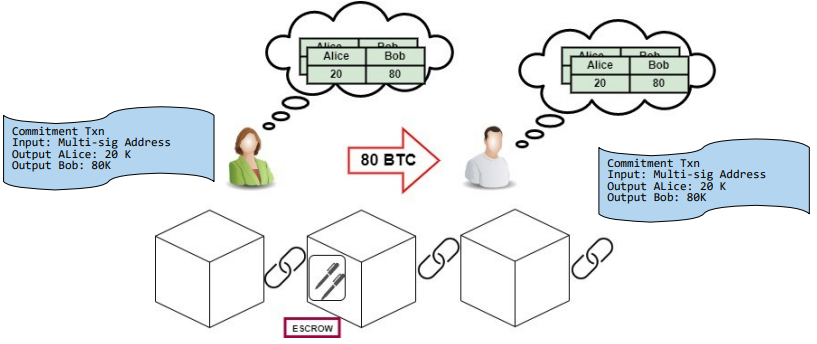
\includegraphics[width=300px]{images/10_Scaling_blockchain/01.png}
    \caption{80 BTC from Alice to Bob}
\end{figure}
but then Bob sends back 10 BTC to Alice, so a new transaction is created, taking data from the multisignature, and exchanged off-chain:
\begin{figure}[H]
    \centering
    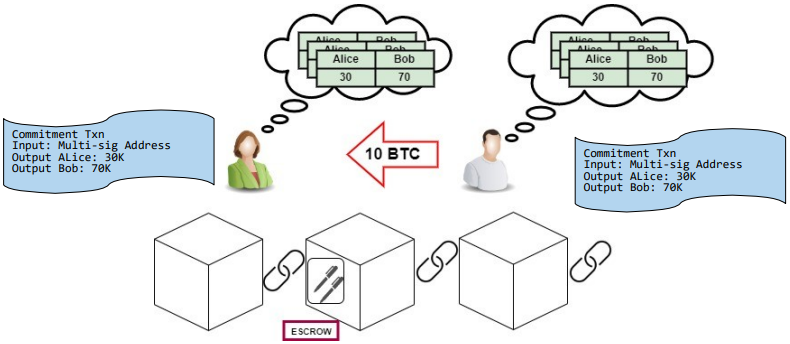
\includegraphics[width=300px]{images/10_Scaling_blockchain/02.png}
    \caption{10 BTC back to Alice}
\end{figure}
Of course every transaction replaces the last one with new updated balances.

Let's suppose now that Bob wants to get their money, so close the channel: he basically has to publish the last transaction on the blockchain who has been signed by both and that's all.
The last transaction exchanged among them is the settle up of all the transactions exchanged between them.

\subsubsection{Double spending protection}
When a transaction is published, Alice or Bob cannot send to the blockchain an older transaction which takes money from the same multi-sig address because it would be rejected from the networ as a double spending (the UTXO is not locked anymore).

\subsubsection{Protection from trapping the funds}
What if Alice funds the multi-sig address and then Bob disappears?
Alice's fund are not trapped in the multi-sig address because to unlock the money both Alice and Bob have to sign the transaction.

To prevent this scam, before publishing the funding transaction Alice asks and wait for Bob transaction in which he sends all the money back to her.
This transaction is taken off-chain and store locally by Alice, constituting a warranty transaction.

It is also possible to insert a hash time lock on the transactions from the counterpart, so if the counterpart disappears Alice can still publish that hash time locked transaction and get her money back in 30 days (for example).

\subsubsection{Protection from previouse transactions publish}
Let's suppose that after a couple of transaction Alice decides to publish on the blockchain a previous transaction, more favourable for her, for example the initial funding transaction.
The transaction is accepted by the blockchain because it was signed both by Alice and Bob.

The network is based around the fact that once you forge or receive a new transaction you drop the old one, but this cannot be enforced by each of the two parts, so a punishment solution has been developed: alongside with a transaction each part sends to the other a \emph{revocation secret}, who has the revocation secret can punish illegal behavior.
So Alice will send, alongside with the new transaction, the revocation secret of it to Bob, and viceversa when Bob creates a new transaction.
If one of the two party publishes a previous transaction, no more valid, the other part can punish him by proving he has the secret and taking all the shares.

An example of that transaction is:
\begin{figure}[H]
    \centering
    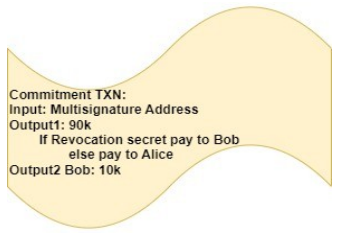
\includegraphics[width=250px]{images/10_Scaling_blockchain/03.png}
    \caption{Commitment transaction with revocation secret}
\end{figure}
If Bob has the revocation secret and Alice publishes one previous transaction more favourable to her Bob ll punish her and take her share.

Of course Bob should be able to do this only for old transaction that are no more valid so Alice reveals a new secret to Bob only whenever she creates a new transaction, sent off-chain and referred to previous transaction.
This basically gives Bob the right to rip up old transactions.

Another thing we need to cope with is that the protocol must give to Bob some time to check if Alice is cheating and to punish her, so Alice must not be able to take money from an older transaction before a time delay.
This can be obtained by modifying the transaction with a time delay:
\begin{figure}[H]
    \centering
    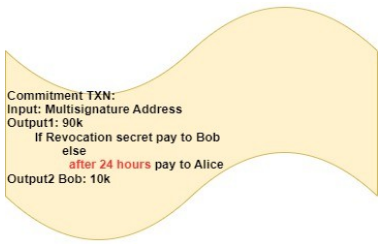
\includegraphics[width=250px]{images/10_Scaling_blockchain/04.png}
    \caption{Commitment transaction with revocation secret and time delay}
\end{figure}

\subsection{Watchtower}
The two parties have to check periodically the blockchain to monitor possible cheating behaviors of the other party because anti-cheating actions must be taken before 1000 blocks have been mined, so at least once a week.
It is possible to let third party to monitor the blockchain on behalf of us.

\subsection{Payment network}
In order to avoid that each person creates a channel to whoever it wants to pay it is possible to exploit the already existing channels.
\begin{figure}[H]
    \centering
    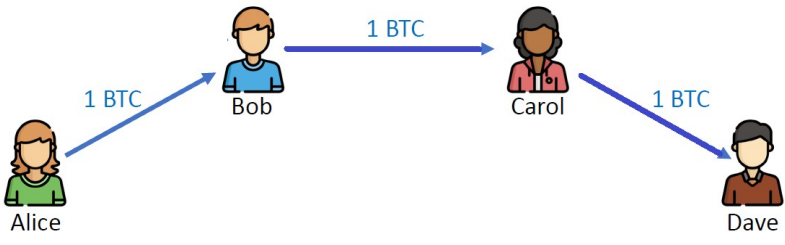
\includegraphics[width=300px]{images/10_Scaling_blockchain/05.png}
    \caption{Payment network}
\end{figure}
Of course we can't trust the nodes in the network so we must protect transactions, again with hash lock and time lock.

Let's suppose that Alice needs to send a payment of 1 BTC to Dave passing through Bob and Carol:
\begin{itemize}
    \item Dave generates a random secret $R$ and the hash $H = H(R)$, then sends $H$ to Alice;
    \item Alice sends a payment of 1BTC to Bob, blocked in a hashed timelock script with the same secret $H$.
    This way Bob can only redeem the funds if he can produce the secret $R$;
    \item each intermediate node then generates a new hashtime lock transaction with the following node, still with the timelock script with $H$;
    \item finally when the path of transaction reaches Dave he can reply with the secret $R$ and redeem it's funds and so on and so forth backward;
    \item when Alice receives $R$ she knows that every one on the path has been payed.
\end{itemize}

If Dave decides not to reveal the secret value $R$ and to not redeem it's fund then each hop can wait for the expire of the hash time lock to get their funds back. 
Also in order to avoid defaulters the time of the time lock should decrease each hop.

\subsection{Routing}
you can pay anyone you can find a route to but it's more complex than that: other than a router you also have to find a route with enough funds on it!

We need a routing protocol that implements:
\begin{itemize}
    \item efficiency: low rate of failures in finding paths, which is the main issue with current algorithms;
    \item privacy: when a node forwards a payment, it should not know where the payment comes from and where the payment is going;
    \item decentralized;
    \item scalability: how many transaction the system can sustain, in term of the size of the network;
    \item balanced channels.
\end{itemize}

The Lightning Network protocol uses source routing which means that the computation of the routing path is left to the sender and it's BGP inspired.
This way each node must have a complete map of the network, which is exploited to compute the path to pursue.
This means that the network performs constant gossip because nodes exchange information on the new channels opened and the one closed, it's a very dynamic network.

\subsubsection{Privacy}
To ensure privacy LN routing implements onion routing (like the Tor one):
\begin{itemize}
    \item Alice prepares a 2-layered onion and sends it to Bob;
    \item Bob can decrypt the first layer and understand which is the hop to whom it has to talk;
    \item Carol does the same and so on until the last hop is reached.
\end{itemize}
This way each node knows the preceding and the next node, but not the other nodes on the path.

\subsubsection{Capacity}
Channel capacity is the total sum of money transferred in a channel with the opening transactions and it's fixed when the channel is opened, while channel balance is how the money is split between the two nodes, this varies dynamically when the two nodes perform transactions.
A node performs route calculation by exploiting the channel capacity but it does not know the channel balance and it is not sure that there will be enough money on the path to forward the payment.

The idea is to try to route with enough capacity, if payment fails you try another route, until the payment succeeds.
This way the failure rate is high: routing takes more than 3 minutes for 5\% of payments.

\subsubsection{Implementation}
There are various independent open source implementations of this protocol:
\begin{itemize}
    \item C-Lightning;
    \item Eclair (Scala);
    \item Lnd (Go);
    \item Ptarmigan (C++);
    \item Rust-Lighting (Rust);
    \item LIT (Python);
    \item Electrum (Python);
    \item ...
\end{itemize}

Implementing some of the various open source RFC-like specifications called BOLT: Basis Of Lightning Technology.

\subsubsection{Open challenges}
There are a lot of open challenges around L2 technologies:
\begin{itemize}
    \item new decentralized, scalable and efficient routing algorithms:
    \begin{itemize}
        \item ant algorithms;
        \item gossip-based.
    \end{itemize}
    \item when new channels should be opened?
    \item what to do when a node is offline? Is it possible to delegate?
    \item atomic multi-path payments: split a payment in multiple path if no feasible path exists;
    \item relation with inter-ledger transfers: atomic swaps of different cryptocurrencies;
    \item monitor the network and construct its topology.
\end{itemize}

Moreover LN needs routing algorithms, it is also not possible to just enter the network because you need to create a payment channel, and to do that you need capital.
Also it's sometime not so practical because longer the route, longer the chances of delay.


